\documentclass[svgnames,tikz]{standalone}
\usepackage{pgfmath}
\usetikzlibrary{positioning,arrows,calc,3d}

\tikzset{
  focus/.style args={#1 at #2}{
    insert path={
      %{ [white] (#2.north east) rectangle (#2.south west)}
      ($(#2.center)!#1!(#2.north east) $) rectangle ($(#2.center)!#1!(#2.south west) $)
    }
  },
  focusout/.style args={#1 at #2}{
    even odd rule,
    insert path={
      (#2.north east) rectangle (#2.south west)
      ($(#2.center)!#1!(#2.north east) $) rectangle ($(#2.center)!#1!(#2.south west) $)
    }
  },
  txt/.style={font=\Large\tt},
  img/.style={
     inner sep=2pt,
     draw,
     label/.append style={font=\small\tt},
  },
}


\begin{document}
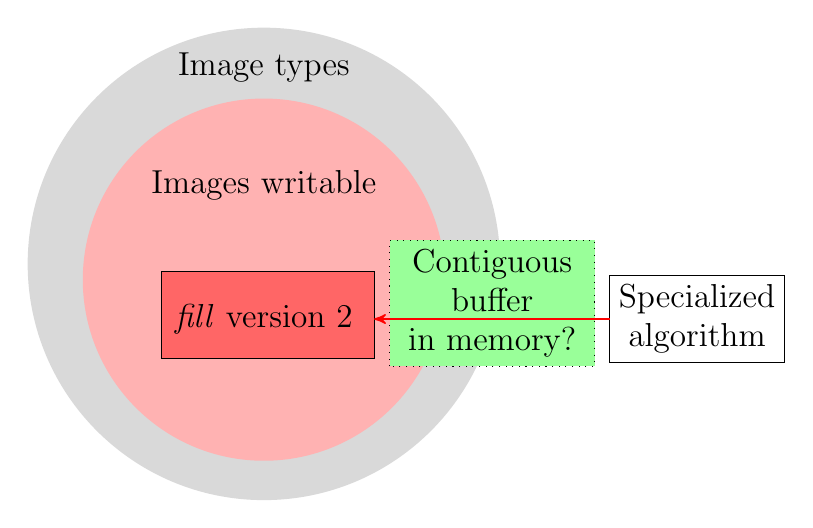
\begin{tikzpicture}
  \tikzset{every node/.style={node distance=5pt, font=\large}}

  \begin{scope}
    \fill[gray!30!white]  (0, 0)    circle  (3);
    \fill[red!30!white]   (0, -0.2) circle  (2.3);

    \draw[black, fill=red!60!white]           (-1.3, -1.2) rectangle (1.4, -0.1);
    \draw[black, dotted, fill=green!40!white] (1.6, -1.3)  rectangle (4.2, 0.3);
  \end{scope}

  \node at (0, 2.5)   {Image types};
  \node at (0, 1)     {Images writable};
  \node at (0, -0.7)  {\emph{fill} version 2};

  \node at (2.9, -0.5) [align=center]       {Contiguous\\ buffer\\ in memory?};
  \node at (5.5, -0.7) [draw, align=center] {Specialized\\ algorithm};

  \draw[color=red, <-, >=stealth', semithick] (1.4, -.7) -- (4.39, -.7);

\end{tikzpicture}
\end{document}